\documentclass[english]{beamer}\usepackage[]{graphicx}\usepackage[]{xcolor}
% maxwidth is the original width if it is less than linewidth
% otherwise use linewidth (to make sure the graphics do not exceed the margin)
\makeatletter
\def\maxwidth{ %
  \ifdim\Gin@nat@width>\linewidth
    \linewidth
  \else
    \Gin@nat@width
  \fi
}
\makeatother

\definecolor{fgcolor}{rgb}{0.345, 0.345, 0.345}
\newcommand{\hlnum}[1]{\textcolor[rgb]{0.686,0.059,0.569}{#1}}%
\newcommand{\hlsng}[1]{\textcolor[rgb]{0.192,0.494,0.8}{#1}}%
\newcommand{\hlcom}[1]{\textcolor[rgb]{0.678,0.584,0.686}{\textit{#1}}}%
\newcommand{\hlopt}[1]{\textcolor[rgb]{0,0,0}{#1}}%
\newcommand{\hldef}[1]{\textcolor[rgb]{0.345,0.345,0.345}{#1}}%
\newcommand{\hlkwa}[1]{\textcolor[rgb]{0.161,0.373,0.58}{\textbf{#1}}}%
\newcommand{\hlkwb}[1]{\textcolor[rgb]{0.69,0.353,0.396}{#1}}%
\newcommand{\hlkwc}[1]{\textcolor[rgb]{0.333,0.667,0.333}{#1}}%
\newcommand{\hlkwd}[1]{\textcolor[rgb]{0.737,0.353,0.396}{\textbf{#1}}}%
\let\hlipl\hlkwb

\usepackage{framed}
\makeatletter
\newenvironment{kframe}{%
 \def\at@end@of@kframe{}%
 \ifinner\ifhmode%
  \def\at@end@of@kframe{\end{minipage}}%
  \begin{minipage}{\columnwidth}%
 \fi\fi%
 \def\FrameCommand##1{\hskip\@totalleftmargin \hskip-\fboxsep
 \colorbox{shadecolor}{##1}\hskip-\fboxsep
     % There is no \\@totalrightmargin, so:
     \hskip-\linewidth \hskip-\@totalleftmargin \hskip\columnwidth}%
 \MakeFramed {\advance\hsize-\width
   \@totalleftmargin\z@ \linewidth\hsize
   \@setminipage}}%
 {\par\unskip\endMakeFramed%
 \at@end@of@kframe}
\makeatother

\definecolor{shadecolor}{rgb}{.97, .97, .97}
\definecolor{messagecolor}{rgb}{0, 0, 0}
\definecolor{warningcolor}{rgb}{1, 0, 1}
\definecolor{errorcolor}{rgb}{1, 0, 0}
\newenvironment{knitrout}{}{} % an empty environment to be redefined in TeX

\usepackage{alltt}

%% The most common packages are already included in:
\usetheme{biostat}
%%%%%%%%%%%%%%%%%%%%%%%%%%%%%%%%%%%%%%%%%%%%%%%%%%%%%%%% 

%% Header data: (adjust to your needs:
\def\uzhunit{Master Thesis Biostatistics}             %% if (not) needed comment/uncomment
%\def\uzhunitext{STA480}
\title[Recruitment rate stochasticity at the design
stage of a clinical trial]{Recruitment rate stochasticity at the design
stage of a clinical trial}
%% Optional Argument in [Brackets]: Short Title for Footline

%% The following are all optional, simply comment them
\subtitle{Supervision by Malgorzata Roos}
%\institute{Biostatistics Journal Club}  %% optional
\author{Pilar Pastor}
%\date{\today}
%%%%%%%%%%%%%%%%%%%%%%%%%%%%%%%%%%%%%%%%%%%%%%%%%%%%%%%% 




%%%%%%%%%%%%%%%%%%%%%%%%%%%%%%%%%%%%%%%%%%%%%%%%%%%%%%%% 
\IfFileExists{upquote.sty}{\usepackage{upquote}}{}
\begin{document}
\maketitle
%%%%%%%%%%%%%%%%%%%%%%%%%%%%%%%%%%%%%%%%%%%%%%%%%%%%%%%% 
%% Start with slides here: put them between `\begin{frame}` and `\end{frame}`


\begin{frame}{Why recruitment rates?}

\begin{itemize}
\item Timely recruitment vital to the success of a clinical trial
\item Inadequate number of subjects $\rightarrow$ lack of power
\item Recruitment period too long $\rightarrow$ competing treatments
\item Recruitment of patients varies at each stage 
\item \cite{carter2004application}
\end{itemize}


\end{frame}


\begin{frame}{Target Population}

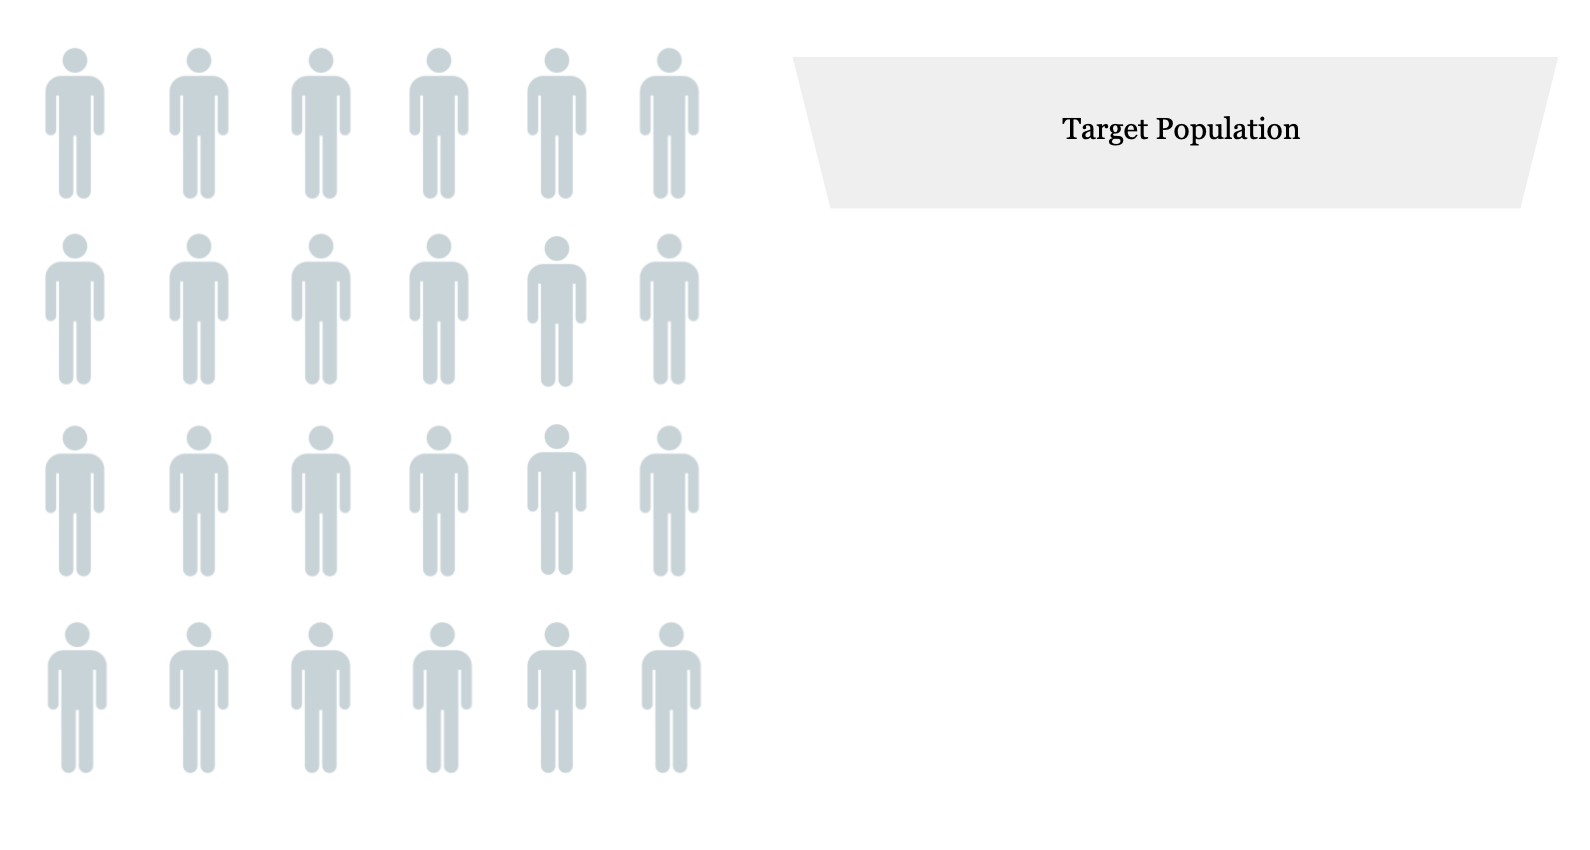
\includegraphics[width=100mm,scale=1]{targetpop.png}

\end{frame}

\begin{frame}{Eligibility}

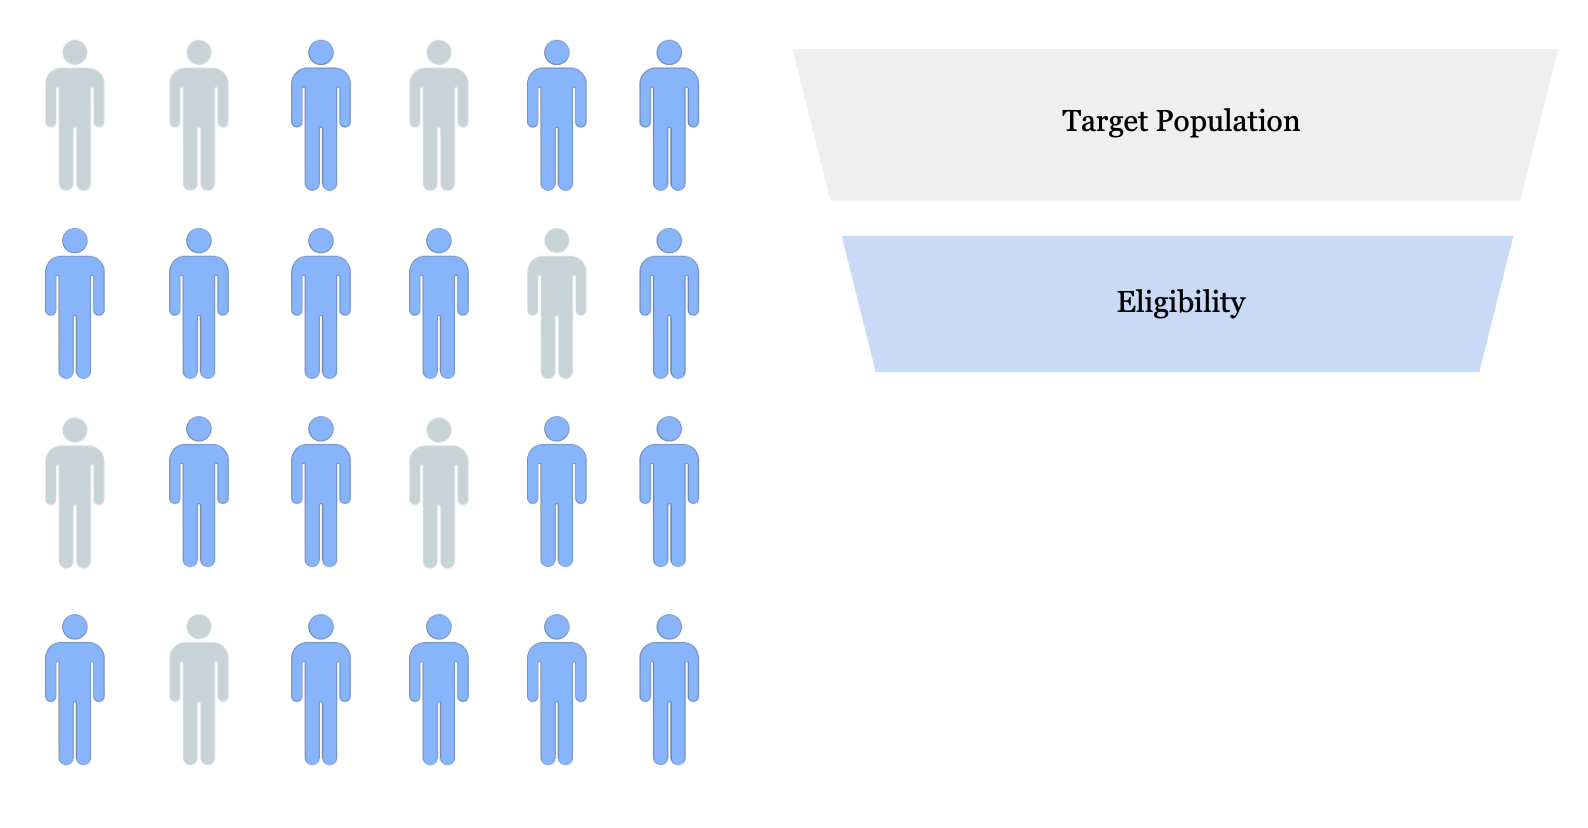
\includegraphics[width=100mm,scale=1]{eligibility.png}

\end{frame}

\begin{frame}{Enrollment}

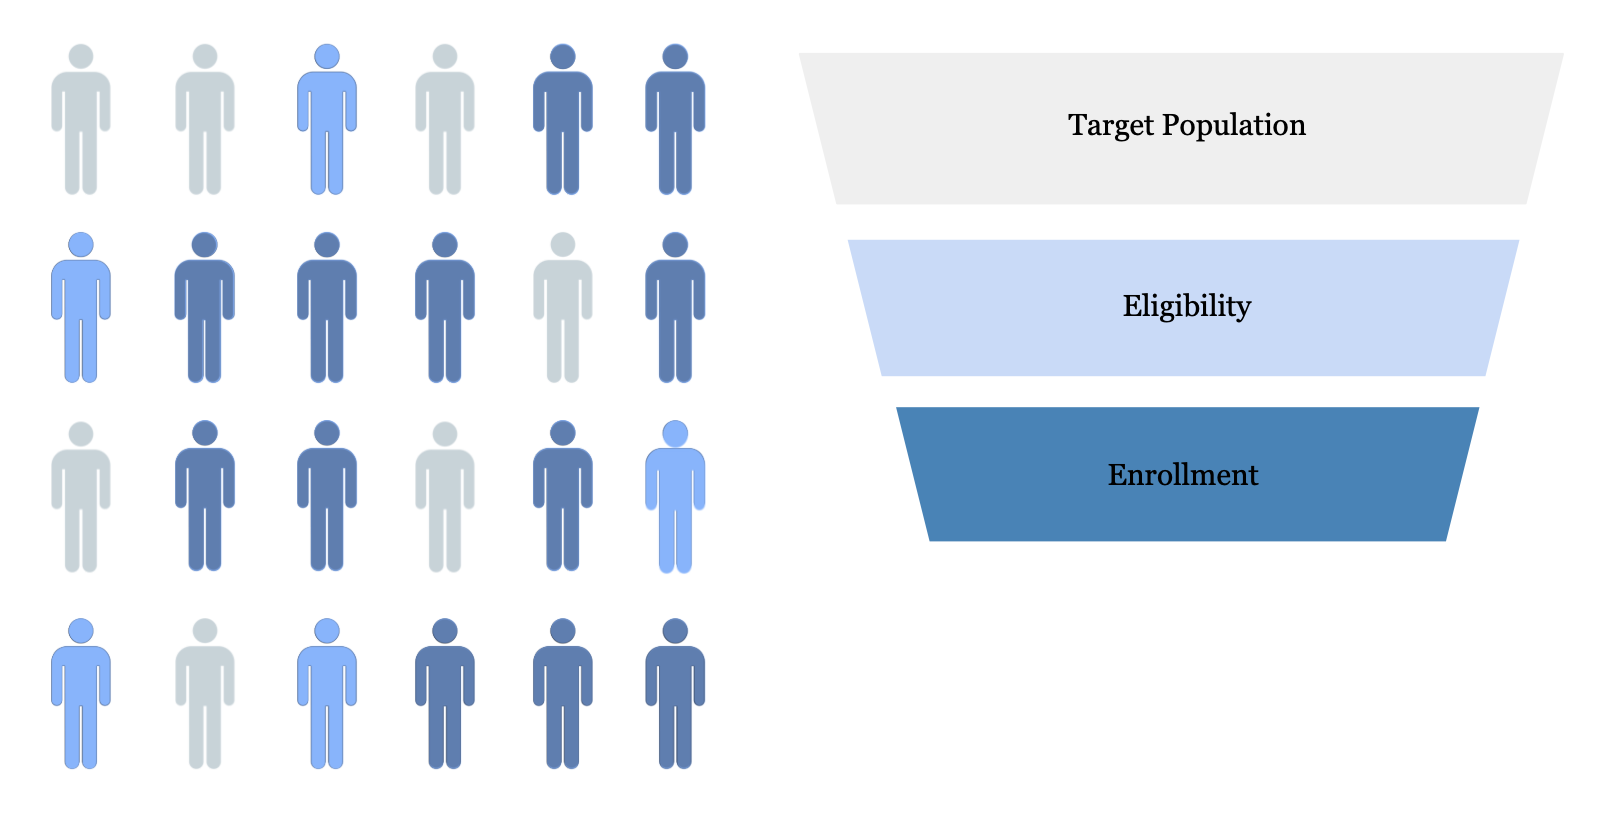
\includegraphics[width=100mm,scale=1]{enrollment.png}


\end{frame}

\begin{frame}{Randomization}

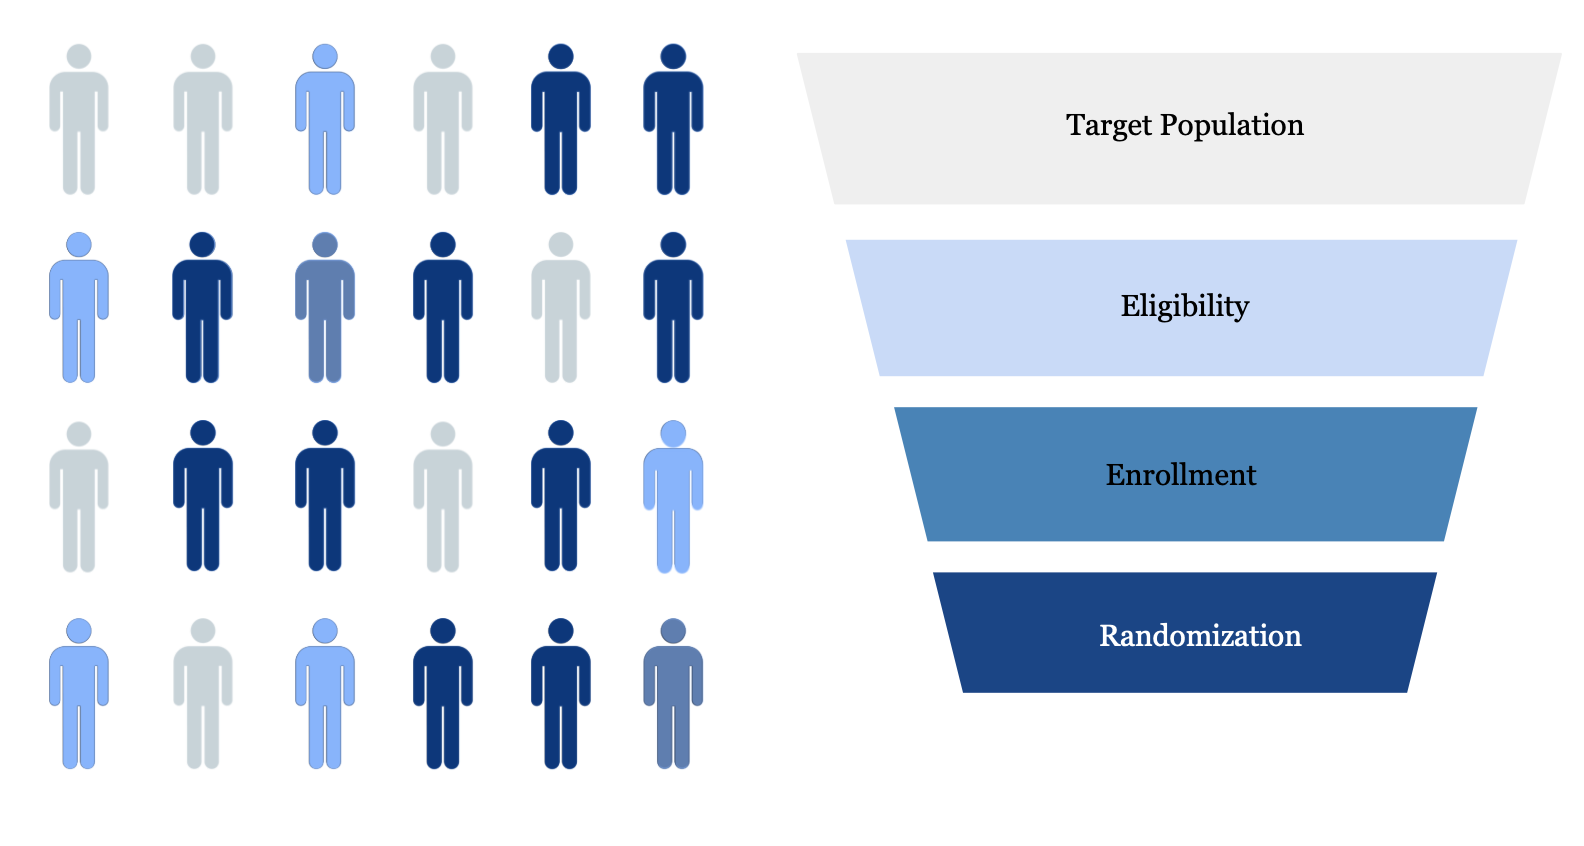
\includegraphics[width=100mm,scale=1]{randomization.png}

\end{frame}

\begin{frame}{Statistical Analysis}

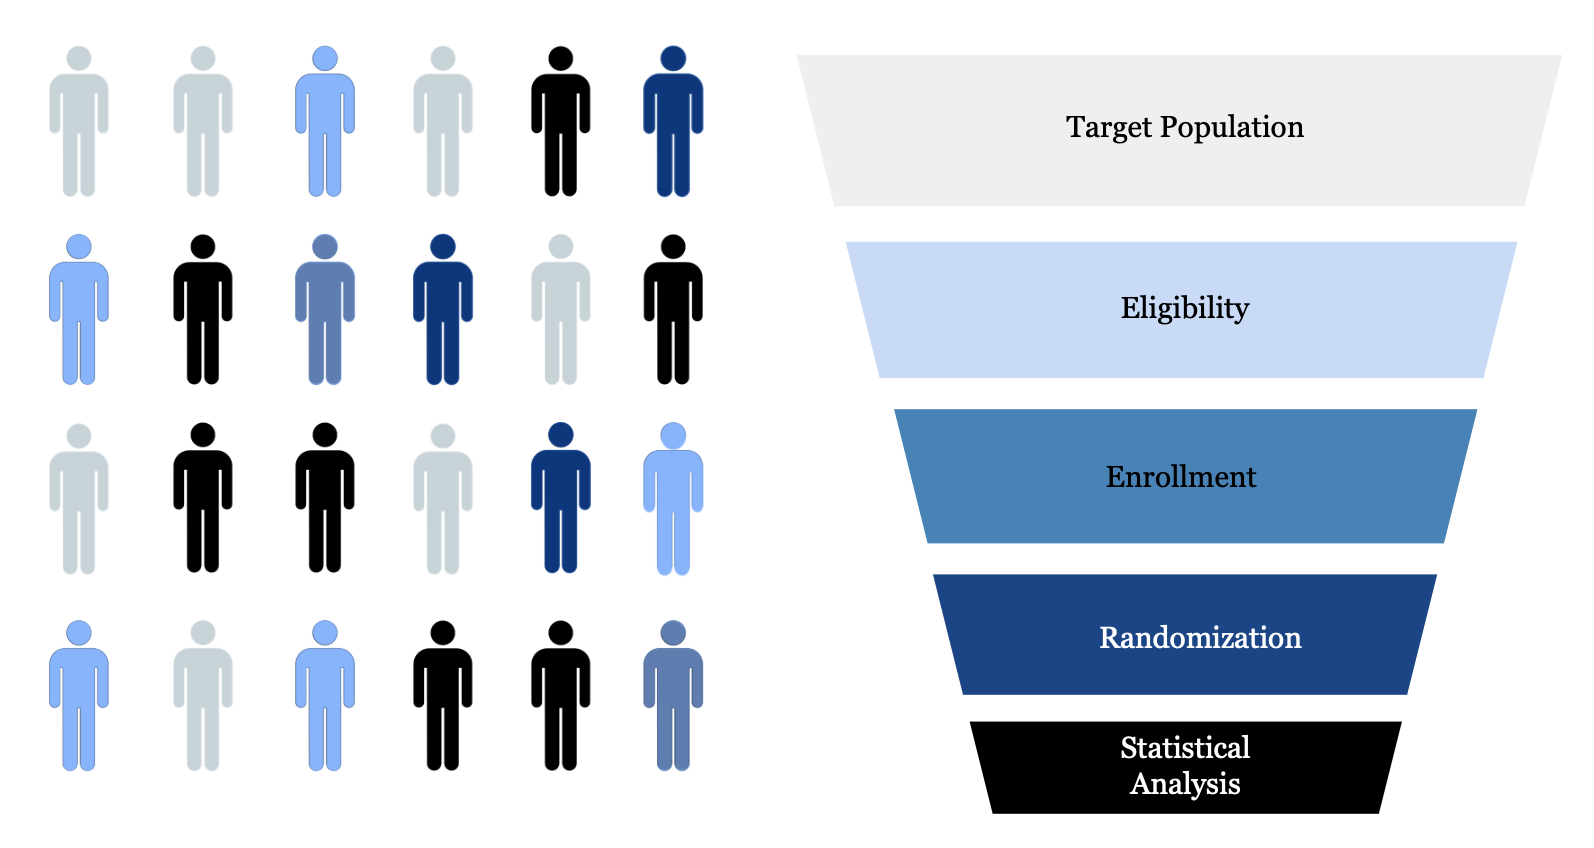
\includegraphics[width=100mm,scale=1]{statanal.png}

\end{frame}


\begin{frame}{Patient Attrition}

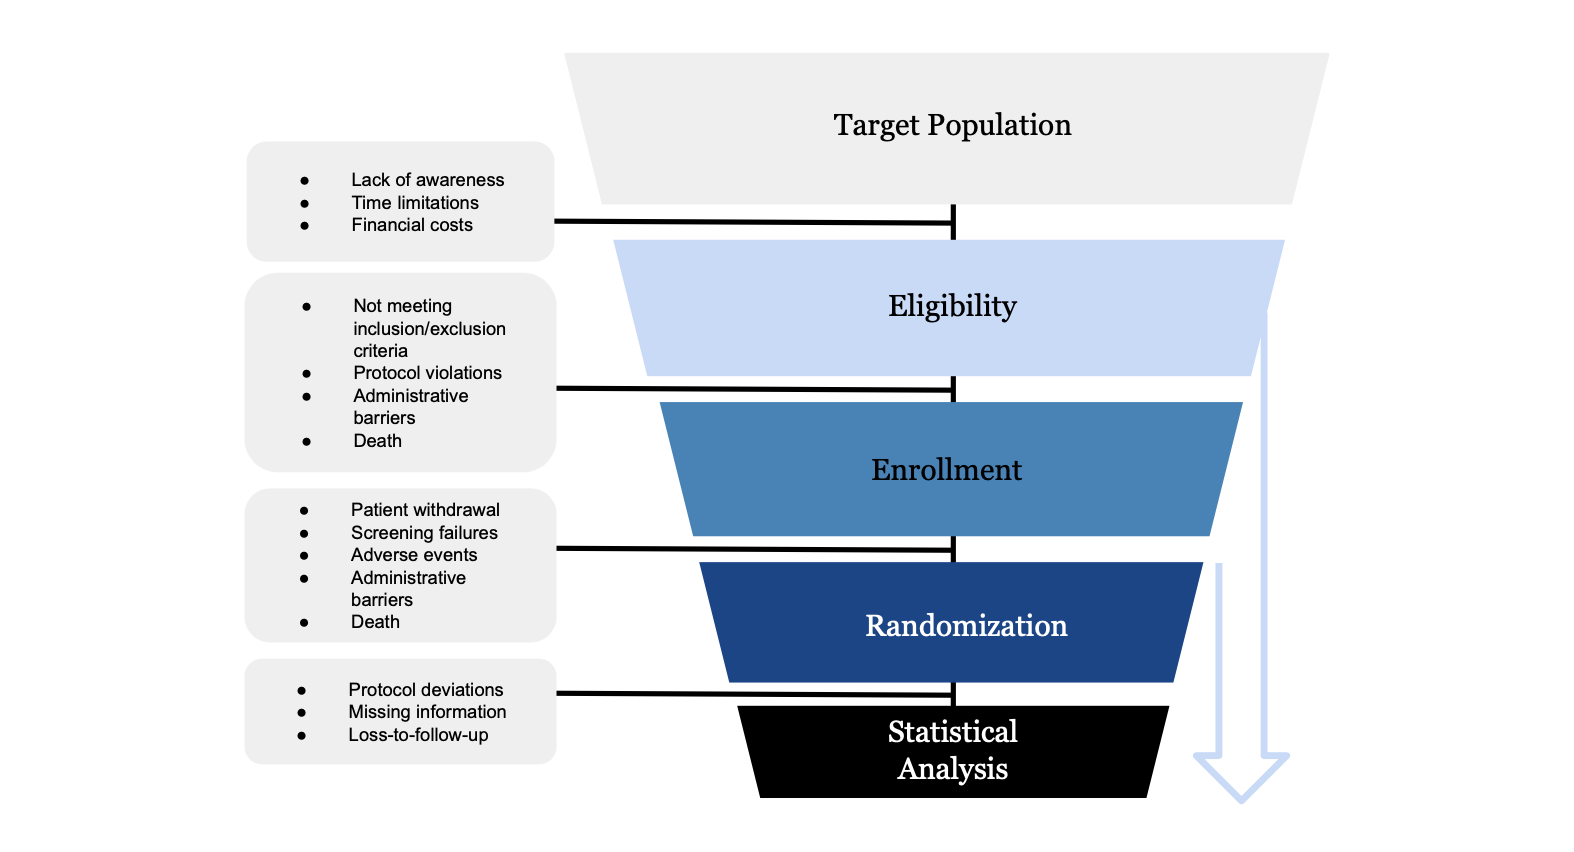
\includegraphics[width=100mm,scale=1]{attrition.png}

\end{frame}

\begin{frame}[shrink = 5]{Shrunk Slide 1}


\end{frame}



\begin{frame}[shrink = 23]{Shrunk slide 2}


\end{frame}



\begin{frame}{Results}


\end{frame}

\begin{frame}{Conclusion}

% 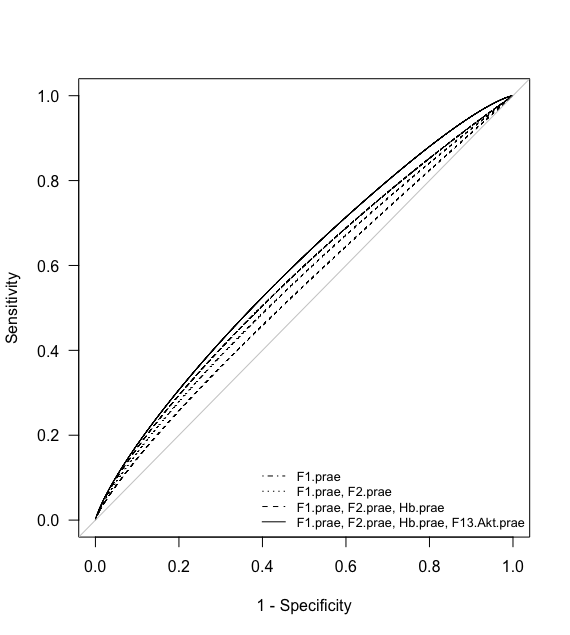
\includegraphics[width=50mm,scale=0.5]{shiftscale6_roc.png}

\end{frame}


\begin{frame}{Next steps}


\end{frame}

\begin{frame}{References}
  \small
  \bibliographystyle{apalike}
\bibliography{illustration}
\end{frame}

%\appendix
%% Possible backup slides...

%% chapter division is accomplished with:
%% \part{Appendix}

\end{document}
